\documentclass{article}

\usepackage{graphicx}
\usepackage{tikz}
\usepackage{tikzsymbols}
\usetikzlibrary{calc,patterns,shapes.geometric}
\pagestyle{empty}
\usepackage[margin=0pt]{geometry}
\geometry{papersize={14in,12in}}

\def\centerarc[#1](#2)(#3:#4:#5){\draw[#1] ($(#2)+({#5*cos(#3)},{#5*sin(#3)})$) arc (#3:#4:#5);}

\begin{document}
	\begin{figure}
		\centering
		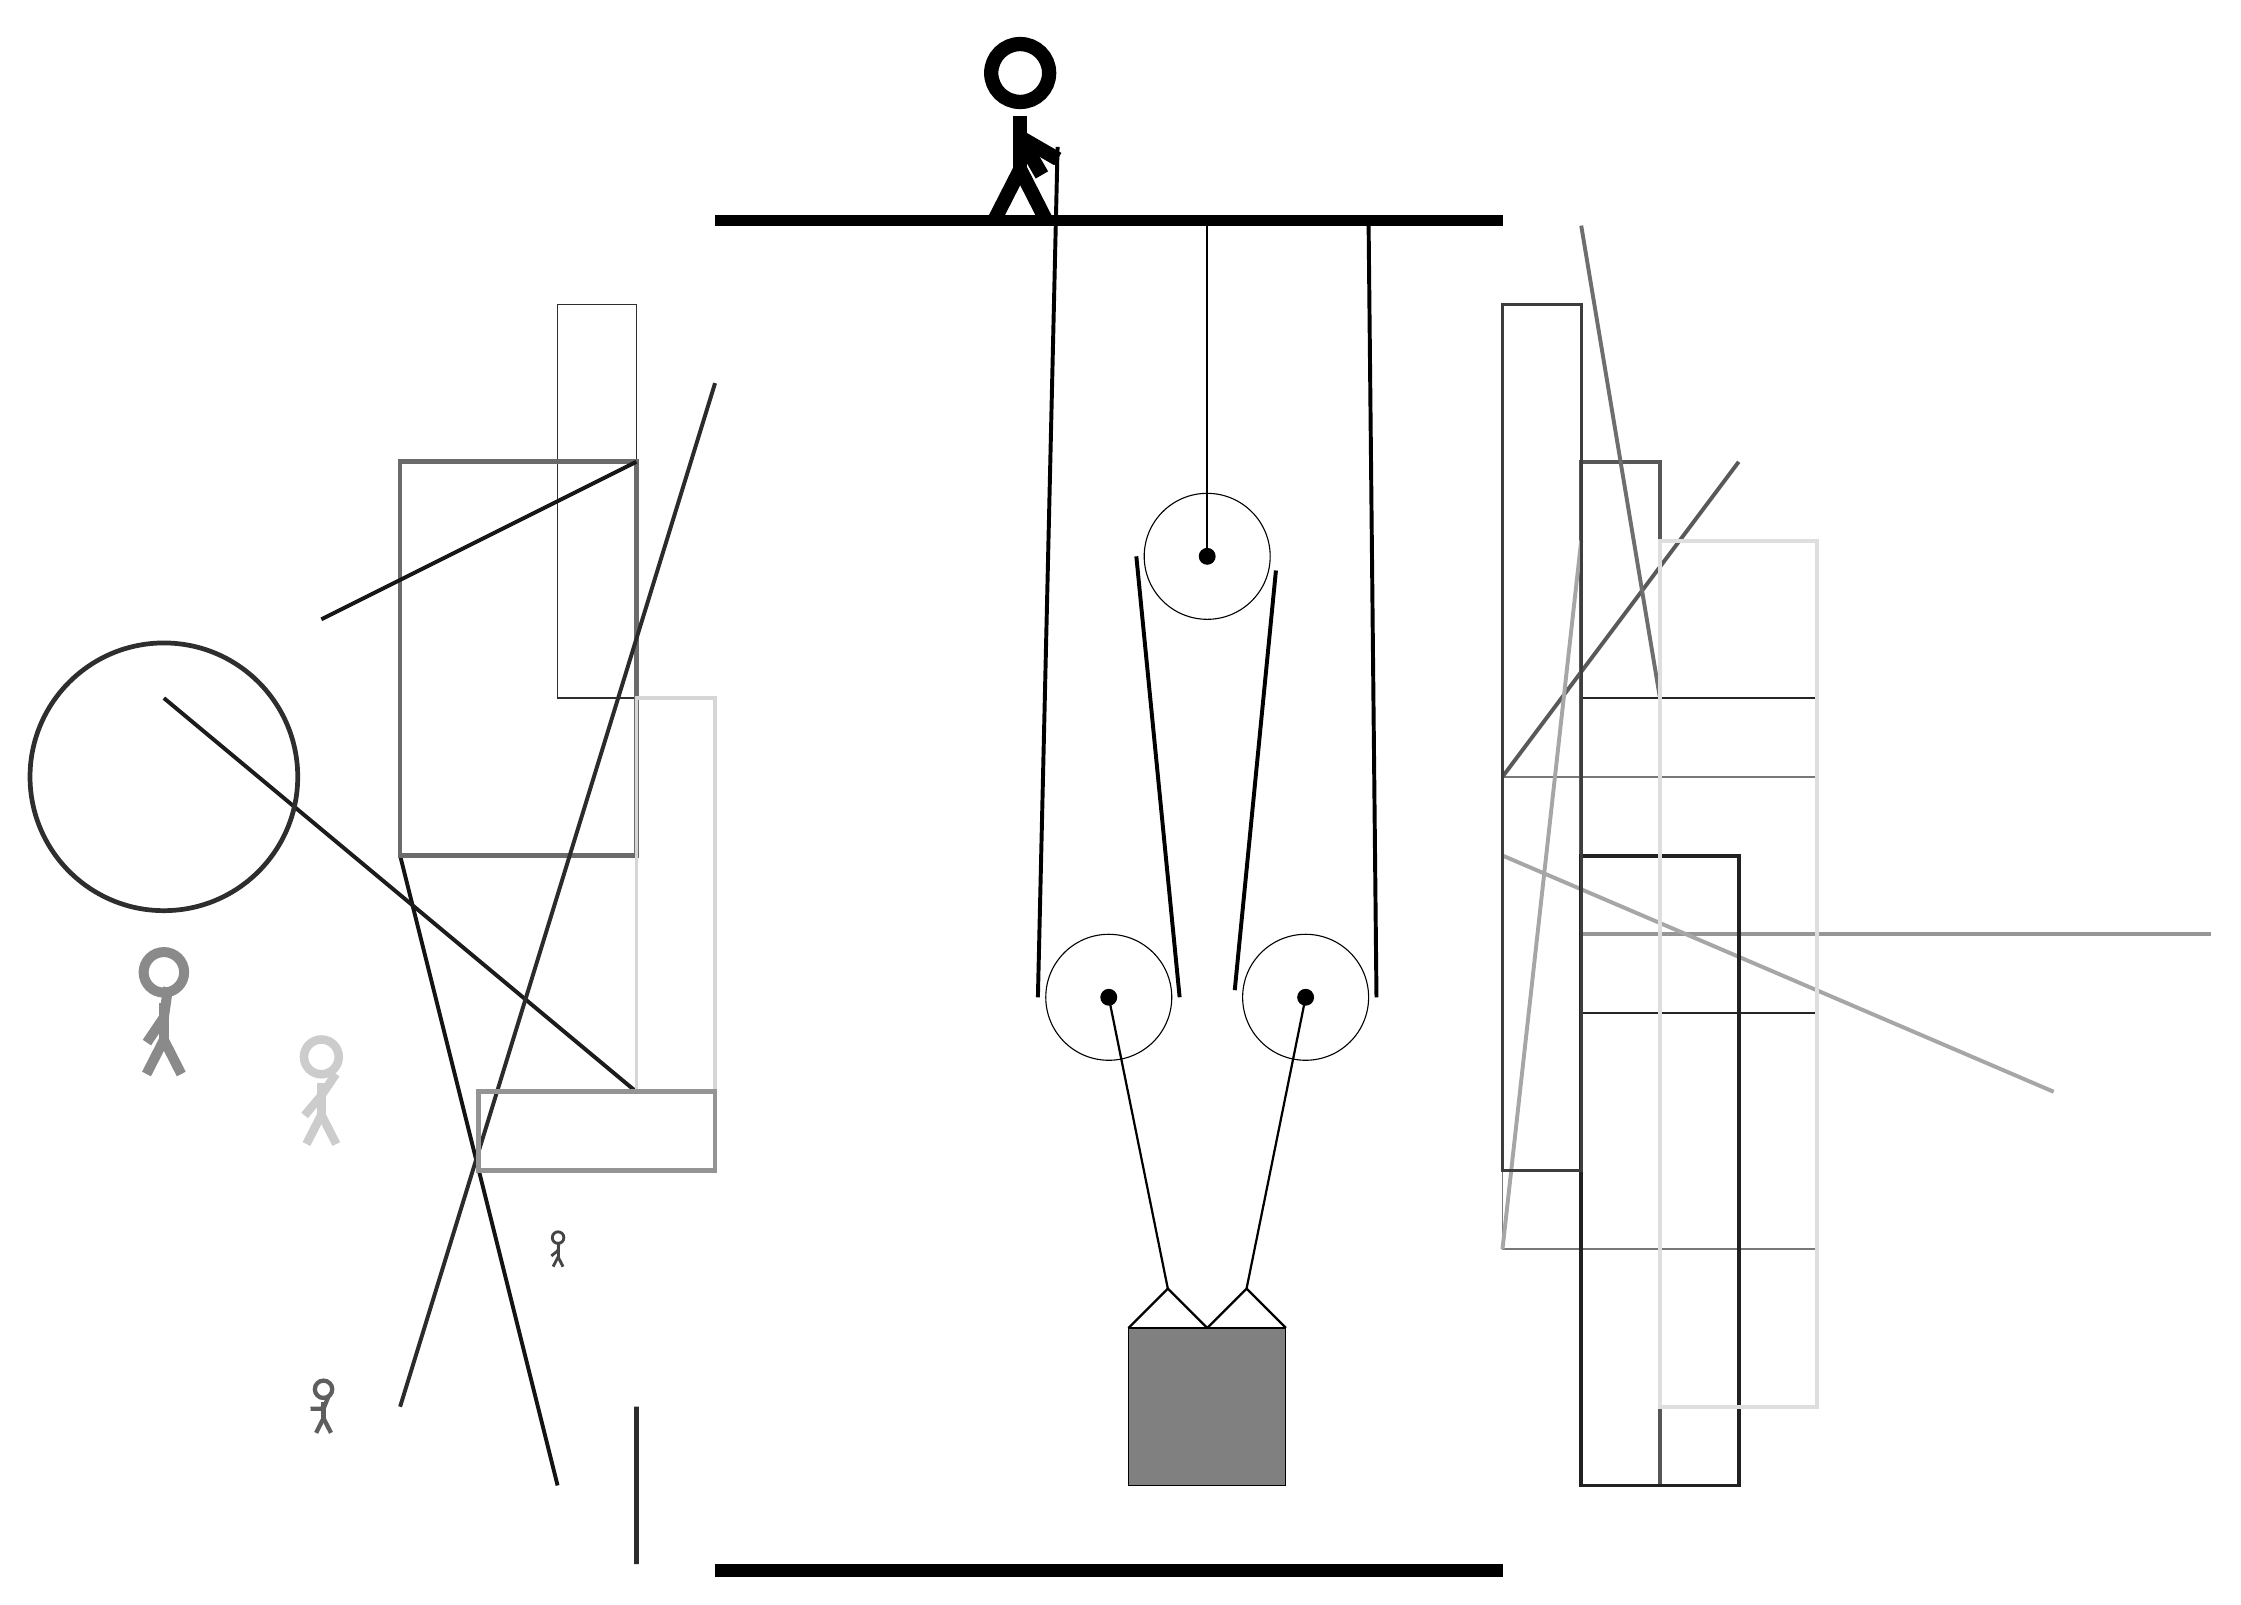
\begin{tikzpicture}
			%%%%% START %%%%%
			
			\draw[fill=black] (-4, 14) rectangle (6, 14.125);
			
			\draw (1, 4.2) circle (0.8);
			\draw[fill=black] (1, 4.2) circle (0.1);
			
			\draw[line width=0.5mm, color=black!41](7, 5) -- (15, 5);
			
			\draw[line width=0.2mm, color=black!53] (6, 1) rectangle (10, 7);
			\draw[line width=0.5mm, color=black!92](-6, -2) -- (-8, 6);
			\draw[line width=0.5mm, color=black!89](-5, 3) -- (-11, 8);
			
			\draw[line width=0.5mm, color=black!65](9, 11) -- (6, 7);
			
			\node[line width=0.2mm, color=black!73] at (-6, 1) {\Strichmaxerl[2][39][84]};
			\draw[line width=0.2mm, color=black!85] (7, 4) rectangle (10, 8);
			
			\draw[line width=0.5mm, color=black!35](6, 6) -- (13, 3);
			\draw [line width=0.6mm, color=black!82](-11, 7) circle (1.7);
			\node[line width=0.4mm, color=black!63] at (-9, -1) {\Strichmaxerl[3][1][68]};
			
			\draw[line width=0.5mm, color=black!66] (8, -2) rectangle (7, 11);
			
			\draw[line width=0.2mm, color=black!82] (-5, 13) rectangle (-6, 8);
			\draw[line width=0.6mm, color=black!58] (-5, 11) rectangle (-8, 6);
			
			\node[line width=0.7mm, color=black!46] at (-11, 4) {\Strichmaxerl[7][56][82]};
			\draw[line width=0.4mm, color=black!16] (-4, 3) rectangle (-5, 8);
			\draw[line width=0.5mm, color=black!35](7, 10) -- (6, 1);
			
			\draw[line width=0.5mm, color=black!91](-9, 9) -- (-5, 11);
			\draw[line width=0.5mm, color=black!83](-8, -1) -- (-4, 12);
			\draw[line width=0.6mm, color=black!42] (-4, 3) rectangle (-7, 2);
			\node[line width=0.7mm, color=black!20] at (-9, 3) {\Strichmaxerl[6][50][56]};
			\draw[line width=0.5mm, color=black!57](7, 14) -- (8, 8);
			
			\draw[line width=0.5mm, color=black!87] (7, -2) rectangle (9, 6);
			\draw[line width=0.4mm, color=black!76] (7, 2) rectangle (6, 13);
			\draw[line width=0.7mm, color=black!83] (-5, -1) rectangle (-5, -3);
			\draw[line width=0.5mm, color=black!13] (8, 10) rectangle (10, -1);
			
			
			\draw (2.25, 9.8) circle (0.8);
			\draw[fill=black] (2.25, 9.8) circle (0.1);
			\draw[thick] (2.25, 9.8) -- (2.25, 14);
			
			\draw (3.5, 4.2) circle (0.8);
			\draw[fill=black] (3.5, 4.2) circle (0.1);
			
			\draw[thick] (3.5, 4.2) -- (2.75, 0.5);
			\draw[thick] (1, 4.2) -- (1.75, 0.5);
			\draw[thick]  (1.25, 0) -- (1.75, 0.5) -- (2.25, 0);
			\draw[thick]  (2.25, 0) -- (2.75, 0.5) -- (3.25, 0);
			\draw[fill=black!50] (1.25, 0) rectangle (3.25, -2);
			
			\draw[line width=0.5mm] (0.35, 15) --  (0.1, 4.2);
			\centerarc[line width=0.5mm](1, 4.2)(180:360:0.9);
			\draw[line width=0.5mm] (1.9, 4.2) -- (1.35, 9.8);
			\centerarc[line width=0.5mm](2.25, 9.8)(-20:180:0.9);
			\draw[line width=0.5mm](3.123, 9.62) -- (2.6, 4.29);
			\centerarc[line width=0.5mm](3.5, 4.2)(160:360:0.9);
			\draw[line width=0.5mm](4.4, 4.2) -- (4.3, 14);
			
			\node at (-0.07, 15.2) {\Strichmaxerl[10][120][-30]};
			
			\draw[fill=black] (-4, -3) rectangle (6, -3.15);
			
			%%%%% END %%%%%
		\end{tikzpicture}
	\end{figure}	
\end{document}